\chapter{Topological sort of representations by frequency and comprehensibility}
\section{Design of topological sort}

\subsection{Conceptual Basis}
\subsection{Implementation details}

\section{Total ordering of representations}

\section{Discussion of ordering results}
\subsection{Implications}
\subsection{Opportunities for future work}
\subsection{Threats to validity}

\section{Desirable Representations (RQ3)}
\label{sec:rq3}
To determine the overall trends in the data, we created total orderings on the representation nodes in each equivalence class (Figure~\ref{fig:refactoringTree})  with respect to the community standards (RQ1)  and understandability (RQ2) metrics.

\subsection{Analysis}
At a high level, these total orderings were achieved by building directed graphs with the representations as nodes and edge directions determined by the metrics: patterns and projects for community standards and matching and composition for understandability. Then, within each graph, we performed a topological sort to obtain total node orderings.

The graphs for community support are based on Table~\ref{table:nodeCount} and the graphs for understandability are based on Table~\ref{table:testedEdgesTable}. The following sections describe the processes for building and and topologically sorting the graphs.

\begin{figure}[tb]
\centering
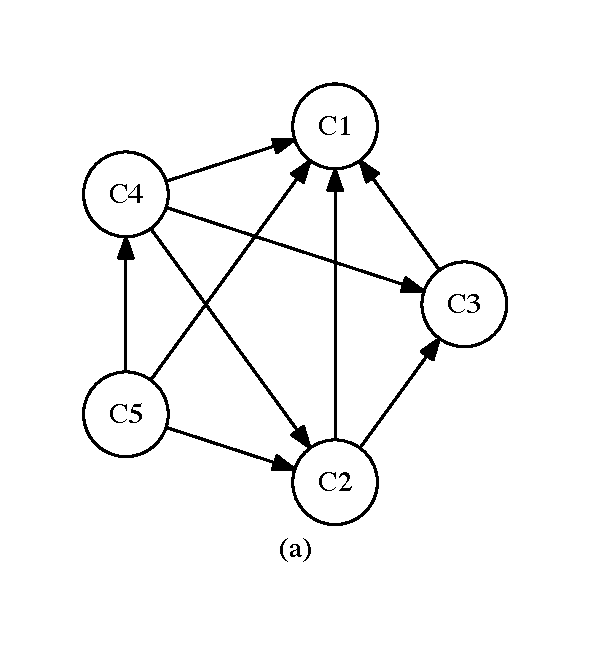
\includegraphics[width=0.42\columnwidth]{nontex/graphs/cart.pdf}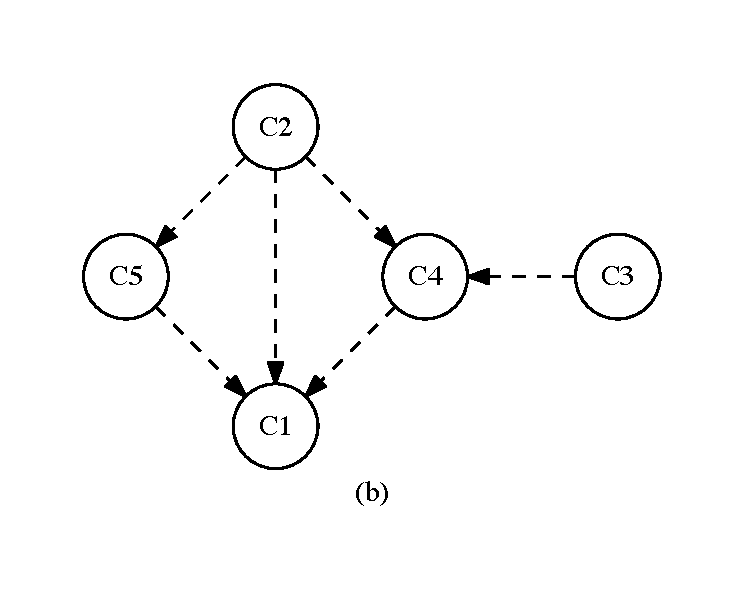
\includegraphics[width=0.57\columnwidth]{nontex/graphs/ccom.pdf}
\vspace{-12pt}
\caption{Trend graphs for the CCC equivalence graph: (a) represent the artifact analysis, (b) represent the understandability analysis.}

\label{fig:graphsforanalysis}
\end{figure}

\todoMid{insert the rest of the graphs?}

\subsubsection{Building the Graphs}
In the community standards graph, we represent a directed edge  $\overrightarrow{C2  C1}$ when  nPatterns(C1) $>$ nPatterns(C2) \emph{and}  nProjects(C1) $>$ nProjects(C2).
When there is a conflict between nPatterns and nProjects, as is the case between L2 and L3 where L2 is found in more patterns and L3 is found in more projects, an undirected edge $\overline{L2L3}$ is used.
This represents that there was no winner based on the two metrics.
After considering all pairs of nodes in each equivalence class that also have an edge in Figure~\ref{fig:refactoringTree}, we have created a graph, for example Figure~\ref{fig:graphsforanalysis}a, that represents the frequency trends among the community artifacts.
Note that with the CCC group, there is no edge between C3 and C5 because there is no straightforward refactoring between those representations, as discussed in Section~\ref{sec:refactoring}.

In the understandability graph, we represent a directed edge  $\overrightarrow{C2C1}$ when match(C1) $>$ match(C2) \emph{and} compose(C1) $>$ compose(C2). When there is a conflict between match and compose, as is the case with T1 and T3 where match(T1) is higher but compose(T3) is higher, an undirected edge $\overline{T1T3}$ is used. When one metric has a tie, as is the case with composition in E9, we resort to the matching metric to determine  $\overrightarrow{C5C1}$. An example understandability graph for the CCC is shown in Figure~\ref{fig:graphsforanalysis}b.

\subsubsection{Topological Sorting}
Once the graphs are built for each equivalence class and each set of metrics, community standards and understandability, we apply a modified version of Kahn's topological sorting algorithm to obtain a total ordering on the nodes, as shown in Algorithm~\ref{topological}. The first modification is to remove all undirected edges since Kahn's operates over a directed graph.

In Kahn's algorithm, all nodes without incoming edges are added to a set $S$ (Line~\ref{addnoincomingtos}), which represents the order in which nodes are explored in the graph. For each $n$ node in $S$ (Line~\ref{beginwhile}), all edges from $n$ are removed and $n$ is added to the topologically sorted list $L$ (Line~\ref{addntoL}). If there exists a node $m$ that has no incoming edges, it is added to $S$.  In the end, $L$ is a topologically sorted list.

\begin{algorithm}
  \caption{Modified Topological Sort}\label{topological}
  \begin{algorithmic}[1]
\State  $L \gets$ []
\State $S \gets$ []
\State Remove all undirected edges (creates a DAG)
\State Add all disconnected nodes to $L$ and remove from graph. If there is more than one, mark the tie. \label{markTie1}
\State Add all nodes with no incoming edges to $S$. If there is more than one, mark the tie. \label{addnoincomingtos}
\While {$S$ is non-empty} \label{beginwhile}
    \State remove a node $n$ from $S$ \label{setn}
    \State add $n$ to $L$  \label{addntoL}
    \For {node $m$ such that $e$ is an edge $\overrightarrow{nm}$}
        \State remove $e$
        \If{$m$ has no incoming edges}
            \State add $m$ to $S$ \label{addToS}
        \EndIf
    \EndFor
    \State If multiple nodes were added to $S$ in this iteration, mark the tie \label{markTie2}
    \State remove $n$ from graph
\EndWhile
\State For all ties in $L$, use a tiebreaker.
  \end{algorithmic}
\end{algorithm}

One downside to Kahn's algorithm is that the total ordering is not unique. Thus, we mark ties in order to identify when a tiebreaker is needed to enforce a total ordering on the nodes. For example, on the understandability graph in Figure~\ref{fig:graphsforanalysis}b, there is a tie between C3 and C2 since both have no incoming edges, so they are marked as a tie on Line~\ref{addnoincomingtos}. Further, when $n=C2$ on line~\ref{setn}, both C5 and C4 are added to $S$ on Line~\ref{addToS}, thus the tie between them is marked on line~\ref{markTie2}. In these cases, a tiebreaker is needed.

Breaking ties on the community standards graph involves choosing the representation that appears in a larger number of projects, as it is more widespread across the community.

Breaking ties in the understandability graph uses the metrics. Based on Table~\ref{table:testedEdgesTable}, we compute the average matching score for all instances of each representation, and do the same for the composition score. For example, C4 appears in E5, E12 and E13 with an overall average matching score of 0.81 and composition score of 24.3. C5 appears in E4 and E9 with an average matching of 0.87 and composition of 28.28. Thus, C5 is favored to C4 and appears higher in the sorting.

\subsection{Results}
After running the topological sort in Algorithm~\ref{topological} with tiebreakers, we have a total ordering on nodes for each graph, shown in Table~\ref{topologicalResults}.  For example, given the graphs in Figure~\ref{fig:graphsforanalysis}a and Figure~\ref{fig:graphsforanalysis}b, the topological sorts are {\tt C1 C3 C2 C4 C5} and {\tt C1 C5 C4 C2 C3}, respectively.

\begin{table*}
\centering
\caption{Topological Sorting, with the left-most position being highest \label{topologicalResults}}
\begin{tabular}{|| l || l || l || l || l || l ||}
                & CCC           & DBB       & LBW & SNG & LIT \\ \hline
Community Standards     & C1 C3 C2 C4 C5    & D2 D1 D3  &  L3 L2 L1     & S2 S1 S3  & T1 T3 T2 T4 \\
Understandability           & C1 C5 C4 C2 C3    & D3 D1 D2  & L3 L2     & S2 S1     & T1 T2 T4 T3 \\
\end{tabular}
\end{table*}


There is a clear winner in each equivalence class, with the exception of DBB.
That is, the node sorted highest in the topological sorts for both the community standards and understandability analyses are C1 for CCC, L3 for LBW, S2 for SNG, and T1 for LIT.
After the top rank, it is not clear who the second place winner is in any of the classes, however, having a consistent and clear winner is evidence of a preference with respect to community standards and understandability, and thus provides guidance for potential refactorings.

This positive result, that the most popular representation in the corpus is also the most understandable, makes sense as people may be more likely to understand things that are familiar or well documented. However, while L3 is the winner for the LBW group, we note that L2 appears in slightly more patterns.

DBB is different  as the orderings are completely reversed depending on the analysis, so the community standards favor D2 and understandability favors D3. Further study is needed on this, as well as on LBW and SNG since not all nodes were considered in the understandability analysis.

